\documentclass{neu_handout}
\usepackage{url}
\usepackage{amssymb}
\usepackage{amsmath}
\usepackage{marvosym}
\usepackage{graphicx}
\usepackage[pdftex]{graphicx}
\usepackage{subfigure}
\graphicspath{ {images/} }
\everymath{\displaystyle}

% Professor/Course information
\title{Milestone 1 - UFOs}
\author{Abby, Emily, Lydia and Peter (The Conspiracists)}
\date{March 2018}
\course{CS 7295}{Information Visualization}

\begin{document}

\section*{1 Data acquisition and clean-up}

\textbf{How dirty was the data and what kind of clean-up was required? How
easy was it to download / use API? What is the format of the data? What are the
items and attributes in your dataset? What types of data are you working with
(categorical, ordinal, quantitative)?}\\

We acquired the data easily from the Reporting Database of the National UFO Reporting Center's website\footnote{Raw Data: \url{http://www.nuforc.org/webreports.html}}. The reports are organized in tables which can be accessed by the following indices: Event Date, State, Shape, Date Posted. When organized by dates, the website provides one table for each month. We downloaded the tables for each year into one excel sheet. Since the report form of the website mostly provides the user with a specific set of options for each question, the data set was relatively clean. The attributes of each item, i.e. report, are:

\begin{description}
  \item[$\bullet$ Date] (date and time of sighting) - quantitative
  \item[$\bullet$ City] (city and/or area of the sighting) - categorical
  \item[$\bullet$ State] - categorical
  \item[$\bullet$ Shape] (one of the 21* choices for craft shapes) - categorical
  \item[$\bullet$ Duration] (statement of estimated duration of the sighting in text) - quantitative
  \item[$\bullet$ Summary] (written description and comments on the sighting)
  \item[$\bullet$ Date Posted] (date the report was posted) - quantitative
\end{description}

We noticed that there are some missing values in the attributes Shape and Duration. We only kept the reports regarding sightings in the US since there were only a few reports outside the US and we can assume that these areas would not be well represented. After this, we are left with 4593 reports. We fixed a few obvious mistakes on the states probably caused by miss-clicking the state close to the right one on the drop-down menu. We changed all the craft shapes with value ``Unknown" to missing values, assuming that a missing value and an ``Unknown" value essentially mean the same thing. Finally, since we intend to use Duration as a quantitative attribute, we used the information of the text to derive the duration of the sighting in minutes. For this last part, we used the mean of a range to give a single number of minutes and we had to make some assumptions as to what people perceive as ``a few minutes" or ``several hours" for example. We believe that these assumptions do not alter the data significantly and would not affect our visualizations.


\section*{2 Exploring the data}

\textbf{Any interesting
trends/observations? Any evidence of missing or “dirty” data? Any features or
observations in the data that are confusing or unexpected?}\\

We explored our data in Tableau and Google Explore. We noticed that there are particular dates with a higher number of UFO sightings, such as Dec 22, Jul 4, Dec 9, and Jan 1. Some of these reports could have been caused by celebratory events associated with certain holidays. For the vast majority of the reports, the sighting's duration was at most one hour but in general the range of the durations is very large (one second to 20 years). In addition, most sightings refer to objects with ``Light" or ``Circle" shape and all 20 shapes (except for ``Unknown", which we cleaned) are present. This will probably make it difficult for us to represent this categorical variable. Finally, although the time of a sighting is almost a uniformly distributed variable, there were a lot of sightings occurring at exactly 3:00 am\footnote{*Changing, Chevron, Cigar, Circle, Cone, Cross, Cylinder, Diamond, Disk, Egg, Fireball, Flask, Formation, Light, Other, Oval, Rectangle, Sphere, Teardrop, Triangle, Unknown}.\\




\section*{3 Interview}

\textbf{How did the interview go? What did you learn? What were you surprised by during the interview? Has the interview changed your motivating questions?}\\ 

After some initial trouble communicating with the director of the National UFO database, and trouble with sourcing a line of communication, we had a solid half hour interview with Peter Davenpor \footnote{Interview Notes: \url{https://docs.google.com/document/d/1ejWb30b9zhYVn6H0adOAkQ_ZRSgHtJb8noliHprtfIw/edit}}, Director of the National UFO Reporting Center. Davenport discussed with us many things regarding his database, most notable of which was his role in establishing the data collection method that the Center uses now. Davenport modernized the collection and organization of the data, both retroactively and for use in the future. We were surprised by how much the tone and attitude of the interview subject changed over the course of the scheduling process and interview; initially, Davenport was skeptical of our use of his data and interview. During the interview, it came to light that this was due to him being burned before by major publications and national news outlets. Our interview was incredibly informative but we did not believe that it changed our line of questioning or reasoning in this project.\\


\section*{4 Task analysis}

\textbf{Create a full list of “domain” tasks (i.e., what are the tasks a
user wants to accomplish with the data using your visualization) and translate these into high/mid/low level tasks.}

\begin{table}[h]
\caption{Domain Tasks} % title name of the table
\centering % centering table
\begin{tabular}{c c c} % creating 3 columns
\hline\hline % inserting double-line
 Task & Abstraction & Level \\ [0.5ex]
\hline % inserts single-line

Observe how the UFO \\sightings occur throughout the years &
Analyze/Consume/Present &
High \\[1ex] %space

Observe all UFO sightings of a particular year \\ and specific details (such as shape) & 
Analyze/Consume/Discover & High \\[1ex] %space

Curiosity stimulation &
Analyze/Consume/Enjoy &
High \\[1ex] %space

Look for areas with high number of sightings &
Search/Explore &
Mid \\[1ex] %space


Are there clusters of UFO\\ sightings according to geographic area? &
Cluster &
Low  \\[1ex] %space

Learn details of sighting (e.g. time, shape, description) &
Retrieve Value &
Low \\[1ex] %space

Only see sightings of particular shape &
Filter &
Low \\[1ex] %space

When did the sightings of a particular area \\(e.g. my hometown) occur? &
Filter &
Low \\[1ex] %space

What state has the most sightings? &
Find Extremum &
Low \\[1ex] %space

What date has the most sightings? &
Find Extremum &
Low \\[1ex] %space

Capture the sightings of a particular month &
Analyze/Produce/Record &
High \\[1ex] %space

What is the distribution of the times\\ of the day the sightings occur? &
Characterize Distribution &
Low \\


\hline 
\end{tabular}
\label{tab:PPer}
\end{table}

\subsection*{4.2 Sketches}

\subsubsection*{4.2.1 Abby's}

\begin{figure}[h]
\centering
{
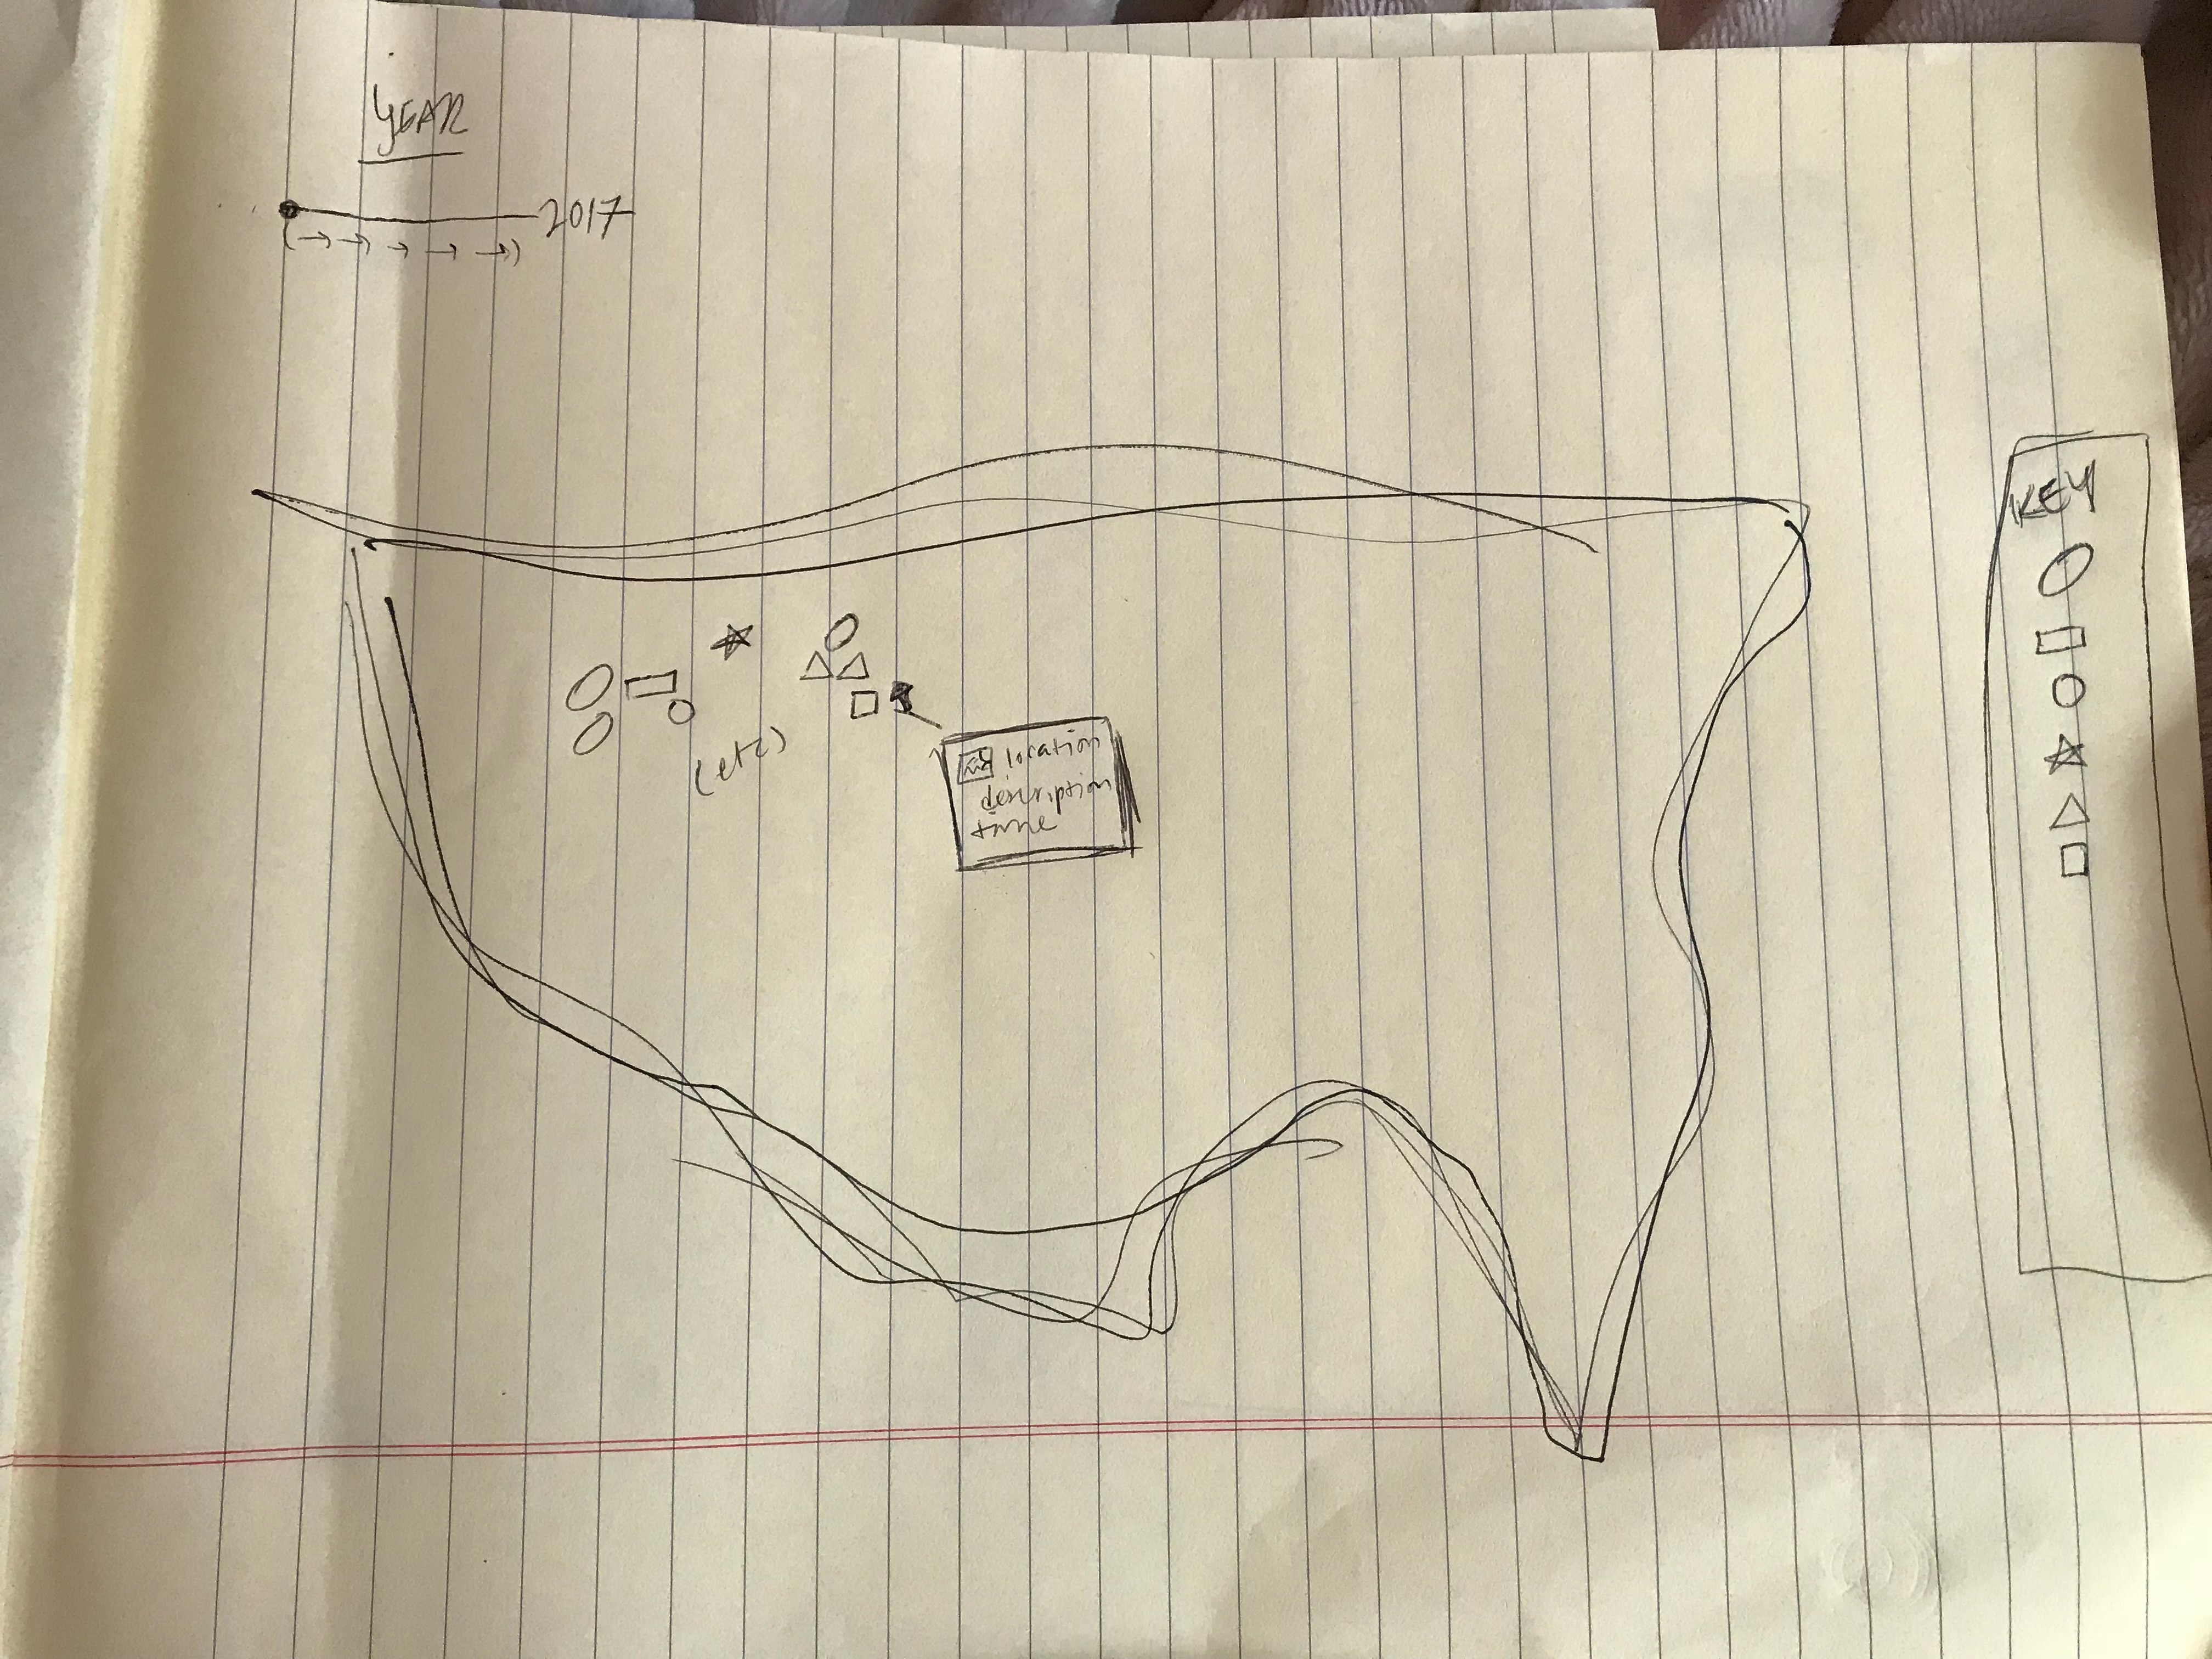
\includegraphics[width=0.9\linewidth]{abby1}
}
\end{figure}

This visualization supports the following tasks: slider on loop, interactive tooltip, populating heat map. The motivations of this is to represent the information in a more journalistic way by using the story features that matter to the reader (it's proximity to them) to attract them to the story. This was my initial idea when I discovered the data set, and has persisted as an option in my mind. 

\newpage

\begin{figure}[h]
\centering
{
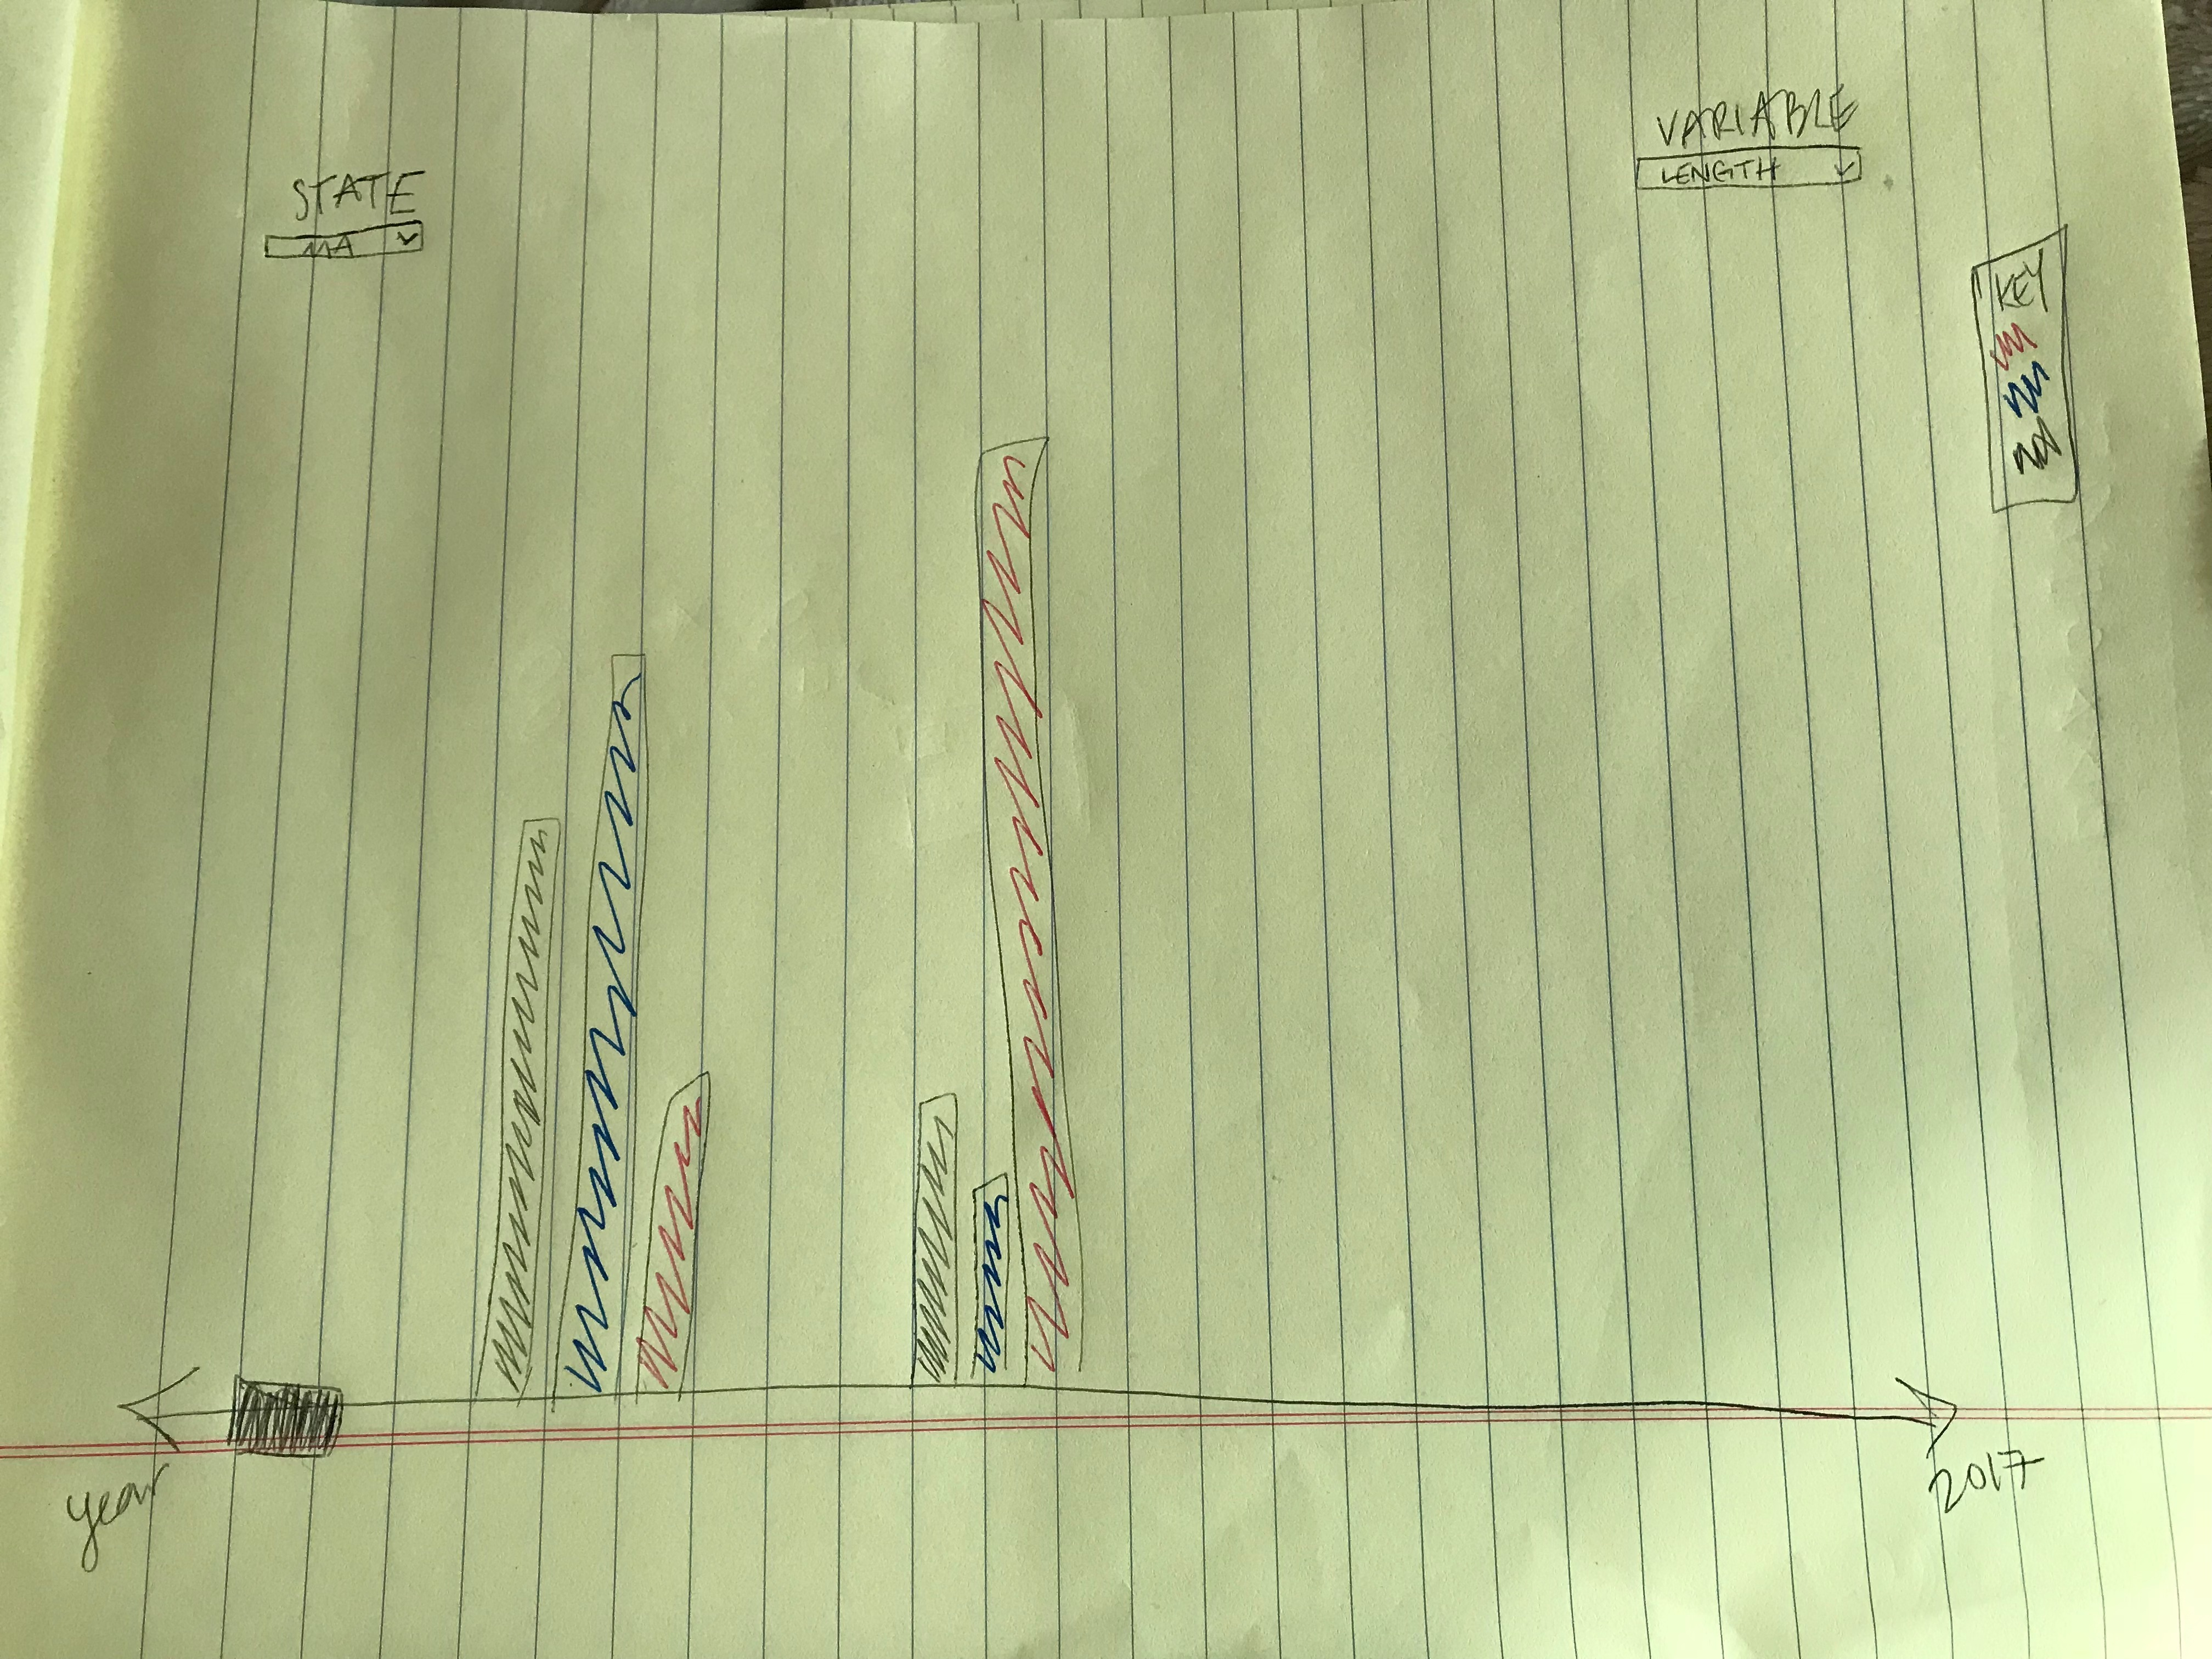
\includegraphics[width=0.9\linewidth]{abby2}
}
\end{figure}

This visualization supports the following tasks: two filters (via drop down menu), interactive timeline, sliding SVG, updating ​side panel. The motivation of this sketch was more of a data-centric approach. The user can explore the data by state via drop down menu, the year, on a sliding timeline and further sort the data by variable: Time occurred, size/shape, etc. Each variable has a bin that is represented by the key; the key changes with the variable, as does the data on the grouped bar chart. This idea is a little more complex but I believe really allows the user to drill down to the specific spot in the data they want.

\newpage

\subsubsection*{4.2.2 Emily's}

\begin{figure}[h]
\centering
{
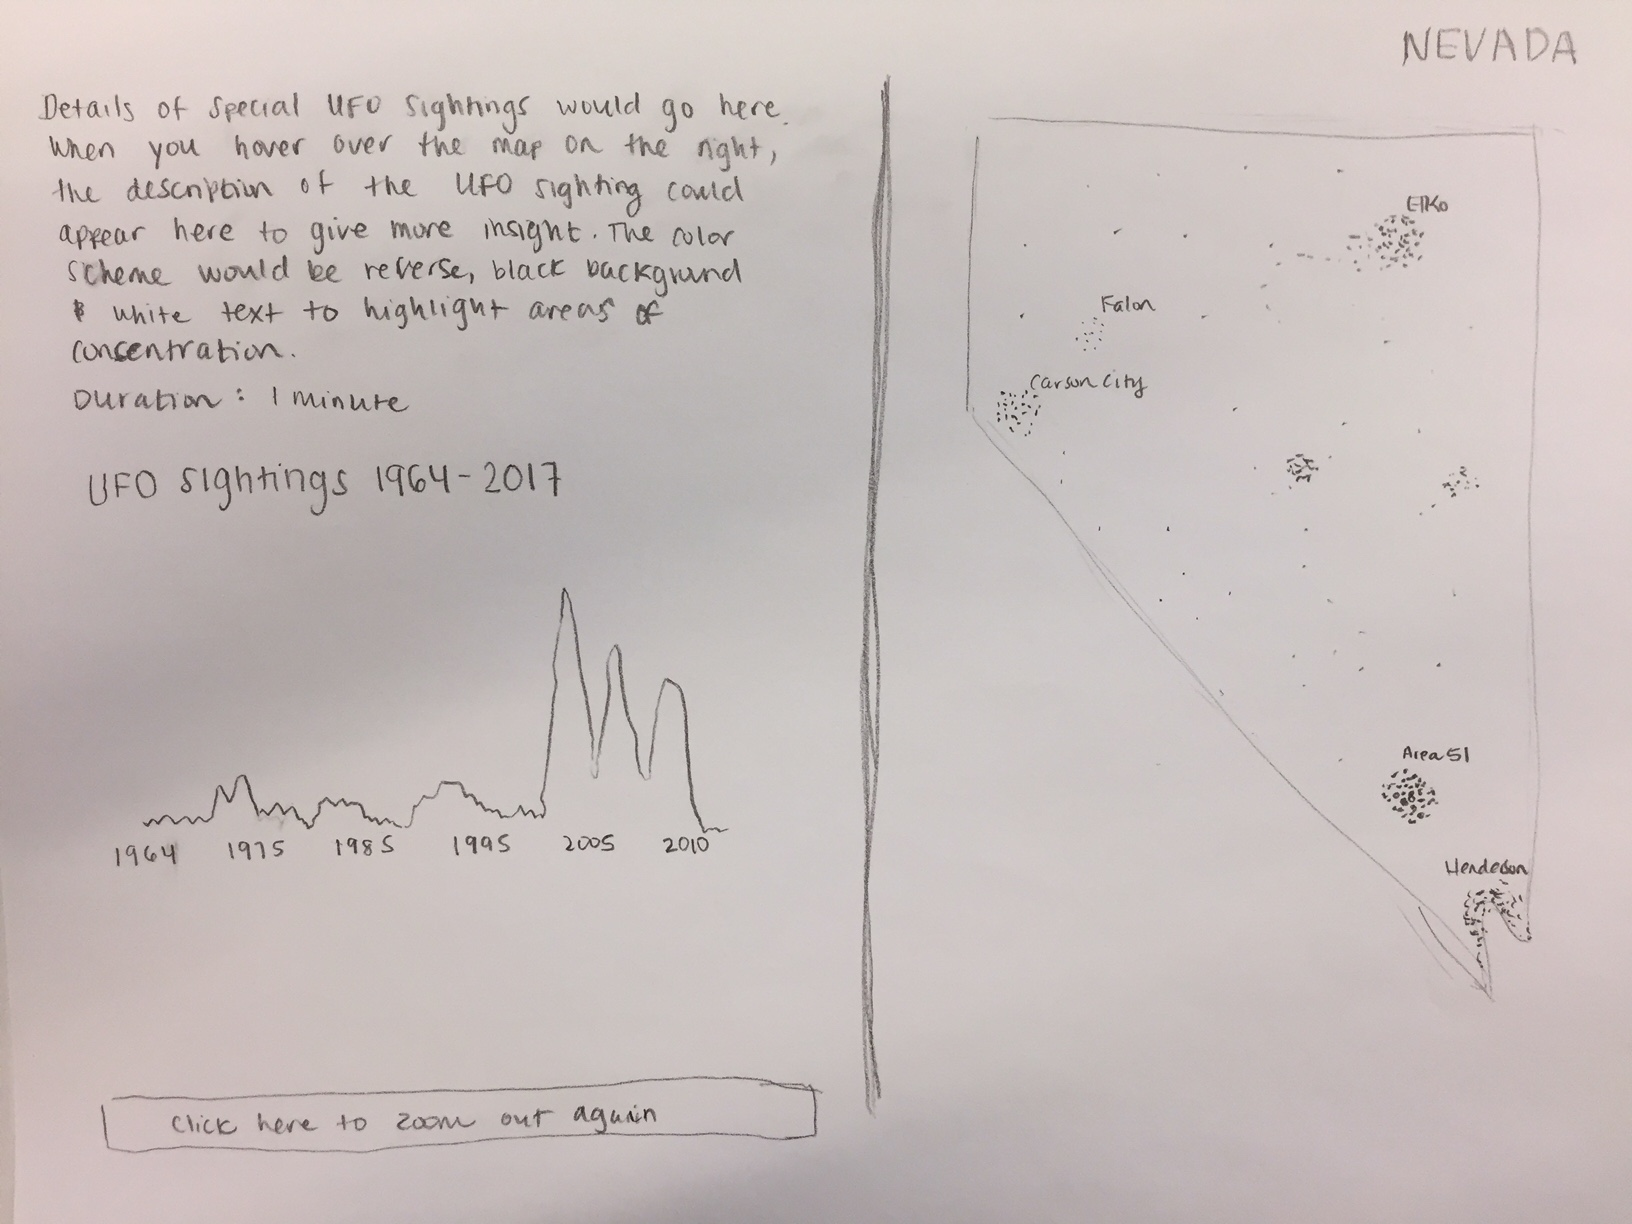
\includegraphics[width=0.9\linewidth]{emily1}
}
\end{figure}

I grouped two visualizations together in this drawing. The idea of this visualization would be able to allow users to select particular states in order to observe all UFO sightings by state. The first visualization should really be a heatmap of the entire U.S., and then this visual is the zoom functionality after a user has selected a state to focus on. Filters could be provided in order to change the time series from all of the data points, to just a particular year. The map of the state (and United States before zooming in) will be used to highlight the number of UFO sightings (showing density), using a black background and white text and encoding to make the number of sightings pop. A line chart would be used to show the quantitative number of sightings, and the detailed description of the UFO sighting would be given above the line chart when a user hovers over a particular data point on the map.\\\\

\newpage

\begin{figure}[h]
\centering
{
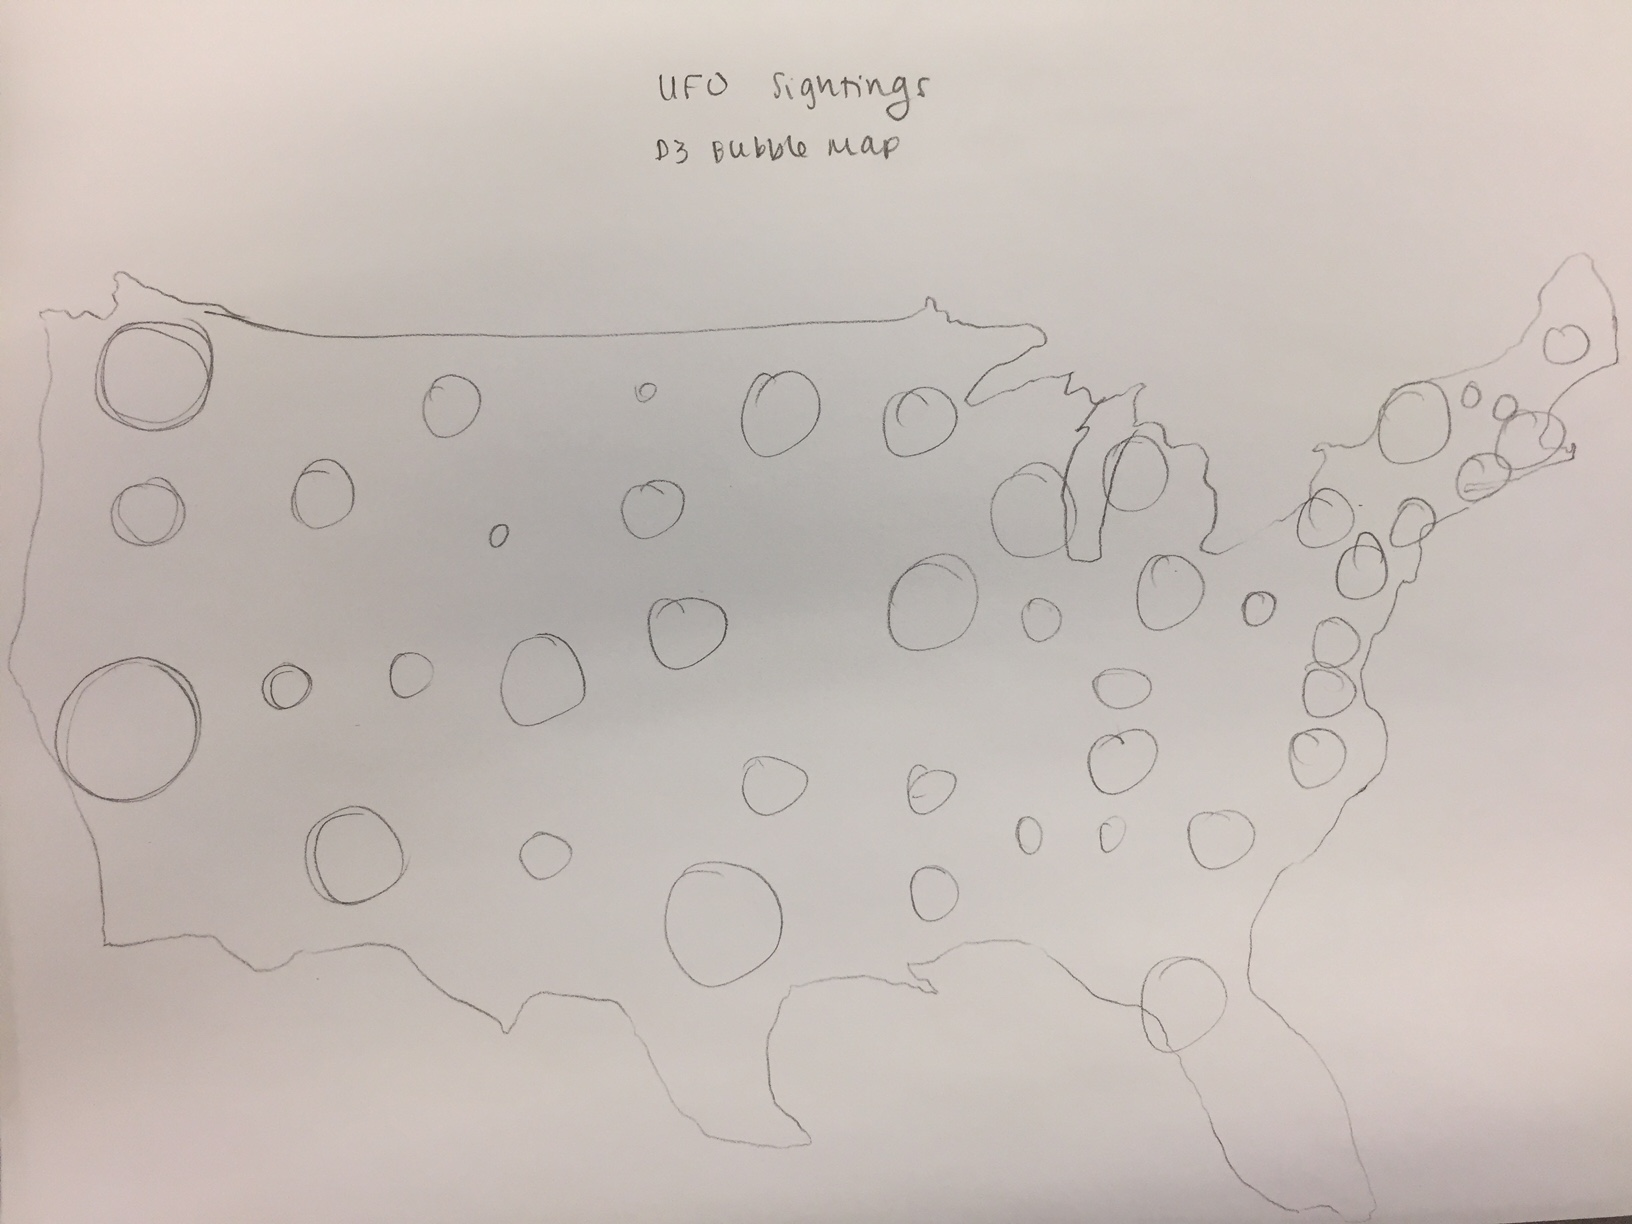
\includegraphics[width=0.9\linewidth]{emily2}
}
\end{figure}

This D3 bubble map would should the total number of reported UFO sightings in the United States by state over the last x number of years (the time range would ideally be filtered by the user). The bubbles would be in a light shaded color in order to make them stand out, and the size of the bubbles would be based upon the number of UFO sightings reported (i.e. 100, 1k, 5, 10k). A legend would be displayed as well.

\newpage

\subsubsection*{4.2.3 Lydia's}

\begin{figure}[h]
\centering
{
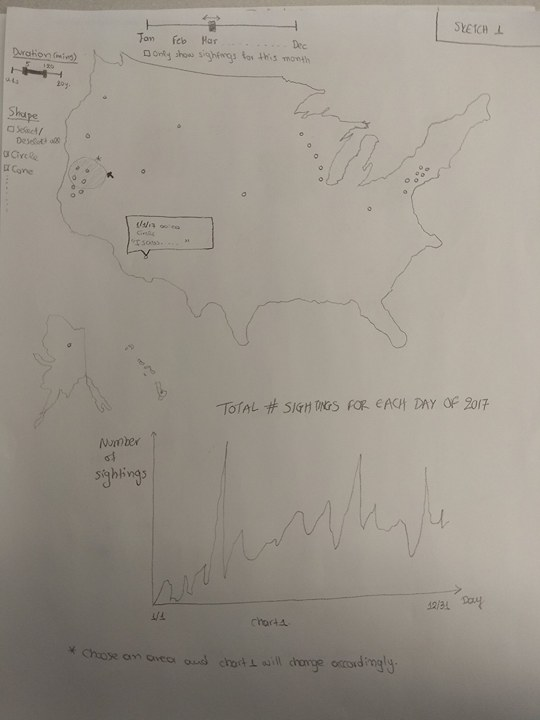
\includegraphics[width=0.7\linewidth]{lydia1}
}
\end{figure}

This visualization supports all tasks except the ``What state has the most sightings?" task. The visual encodings are the map and the line chart. The former is used for most tasks and the latter is used for finding extrema, correlations, and determining ranges. Both are effective for the tasks they support.

\newpage

\begin{figure}[h]
\centering
{
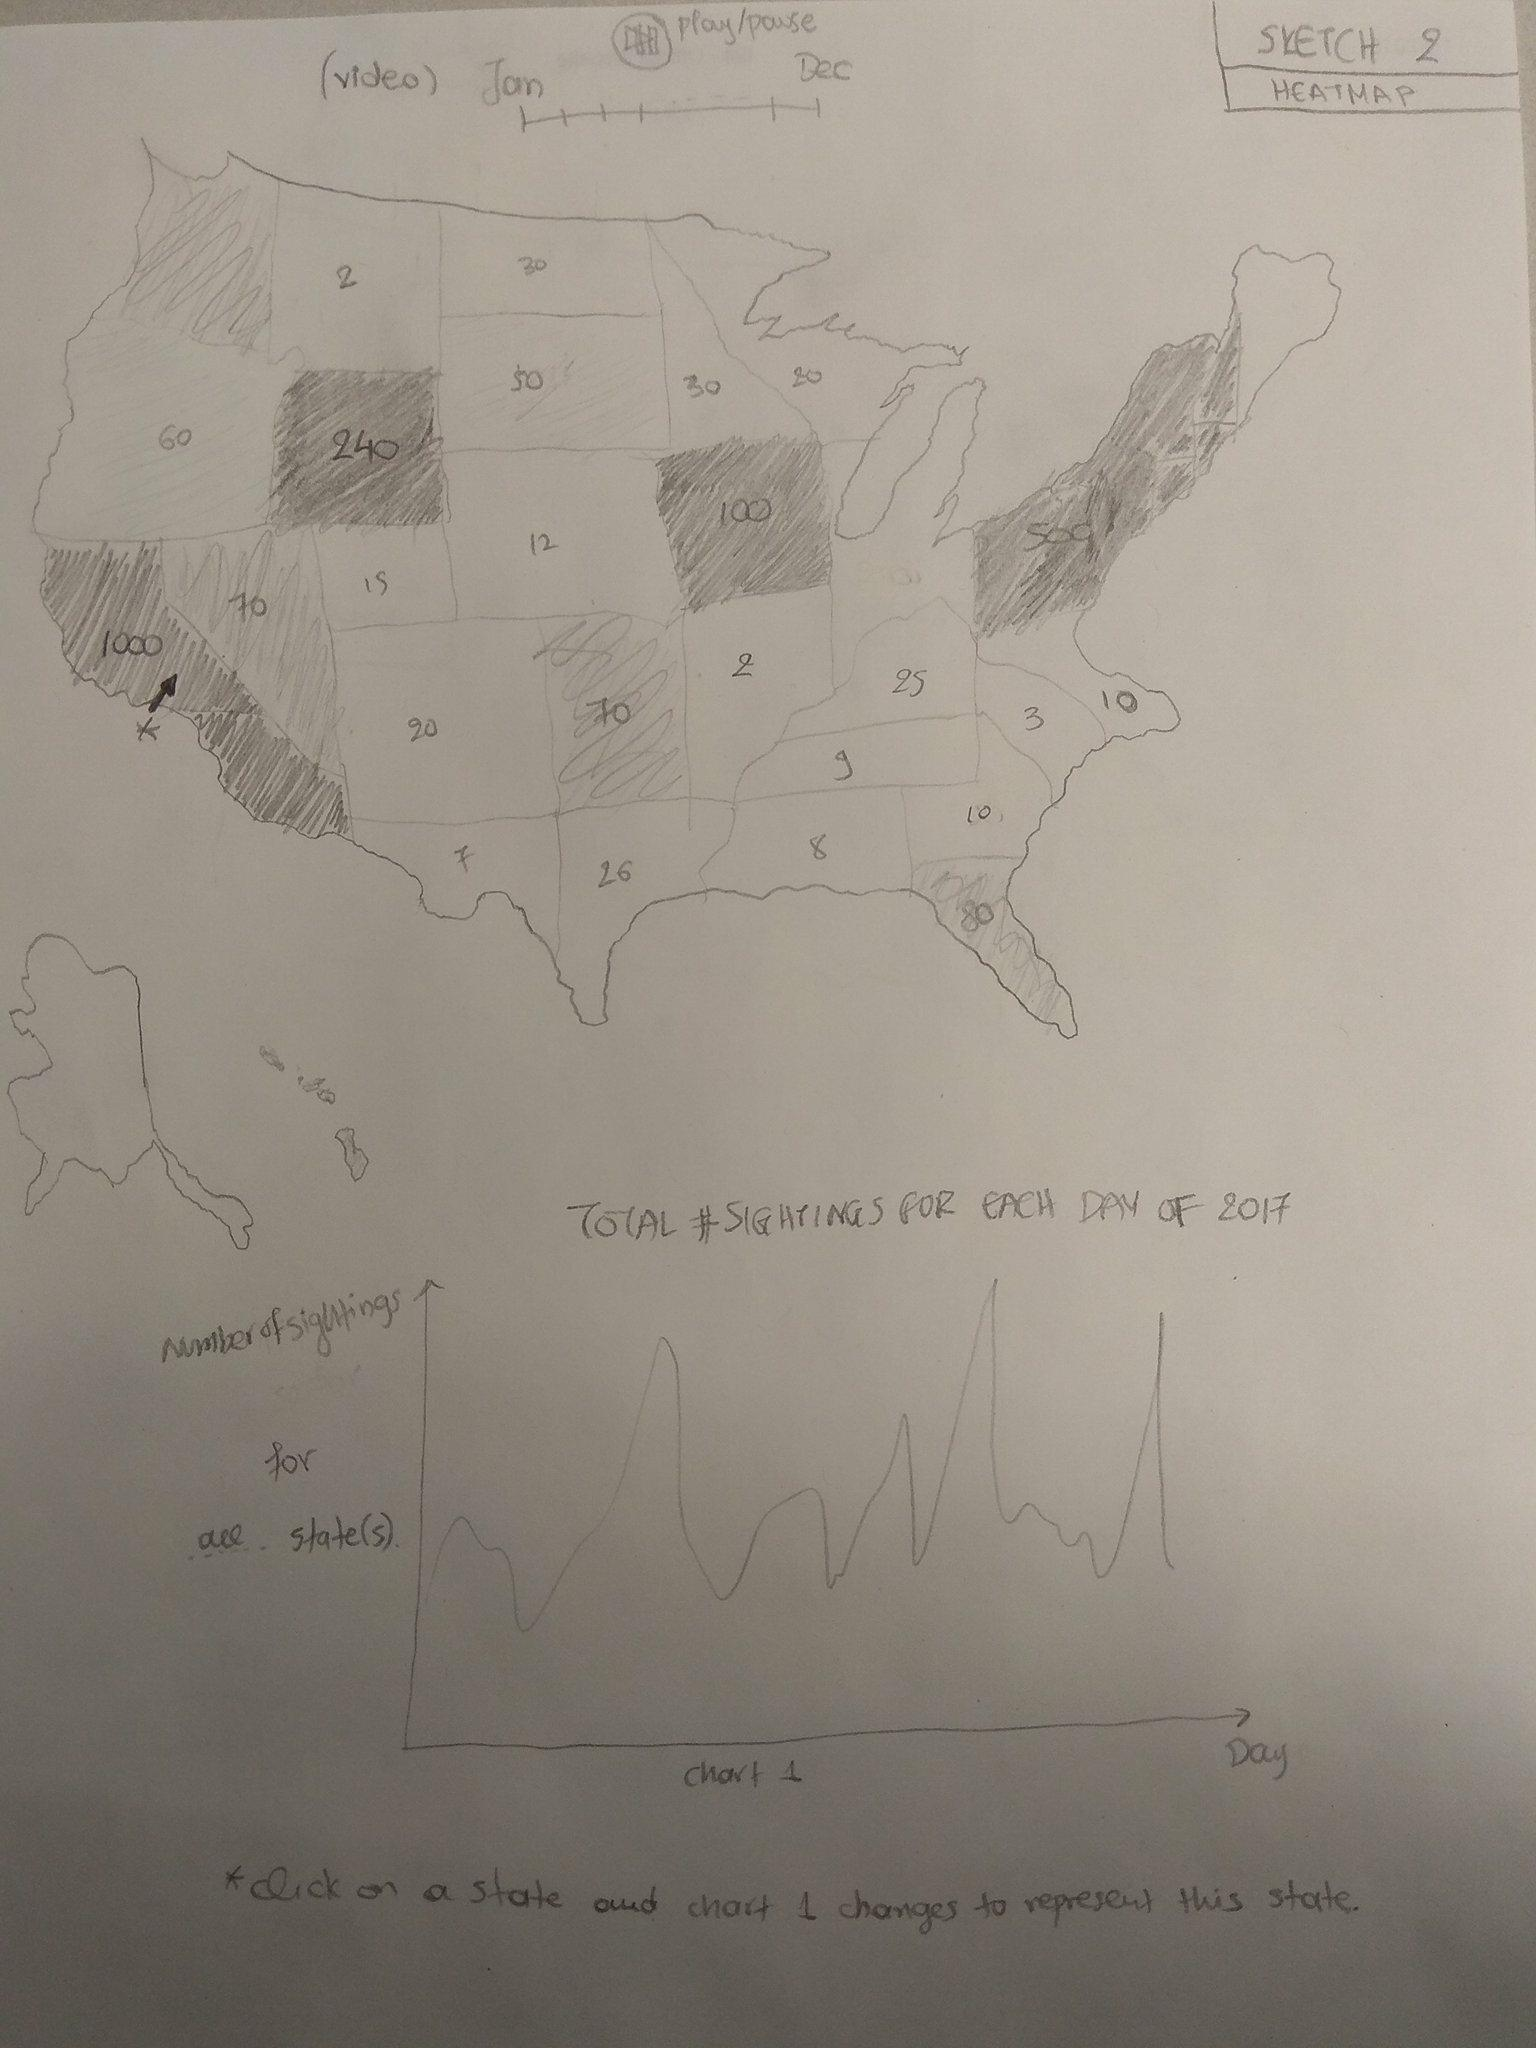
\includegraphics[width=0.7\linewidth]{lydia2}
}
\end{figure}

This visualization focuses on the states, and efficiently supports a task that the other two don't, the ``What state has the most sightings?" task. Using the choropleth map it is easier to approximately identify the ranking of the number of sightings of a state. We could have used a bar chart but the states are too many and geographic data are better represented in a map. The chart helps in finding extrema and correlations as in sketch 1, but this time the selected values could come from different states (instead of different areas selected with the user's mouse). However, this visualization only supports tasks that refer to states and areas (where areas would now only be considered as states).

\newpage

\begin{figure}[h]
\centering
{
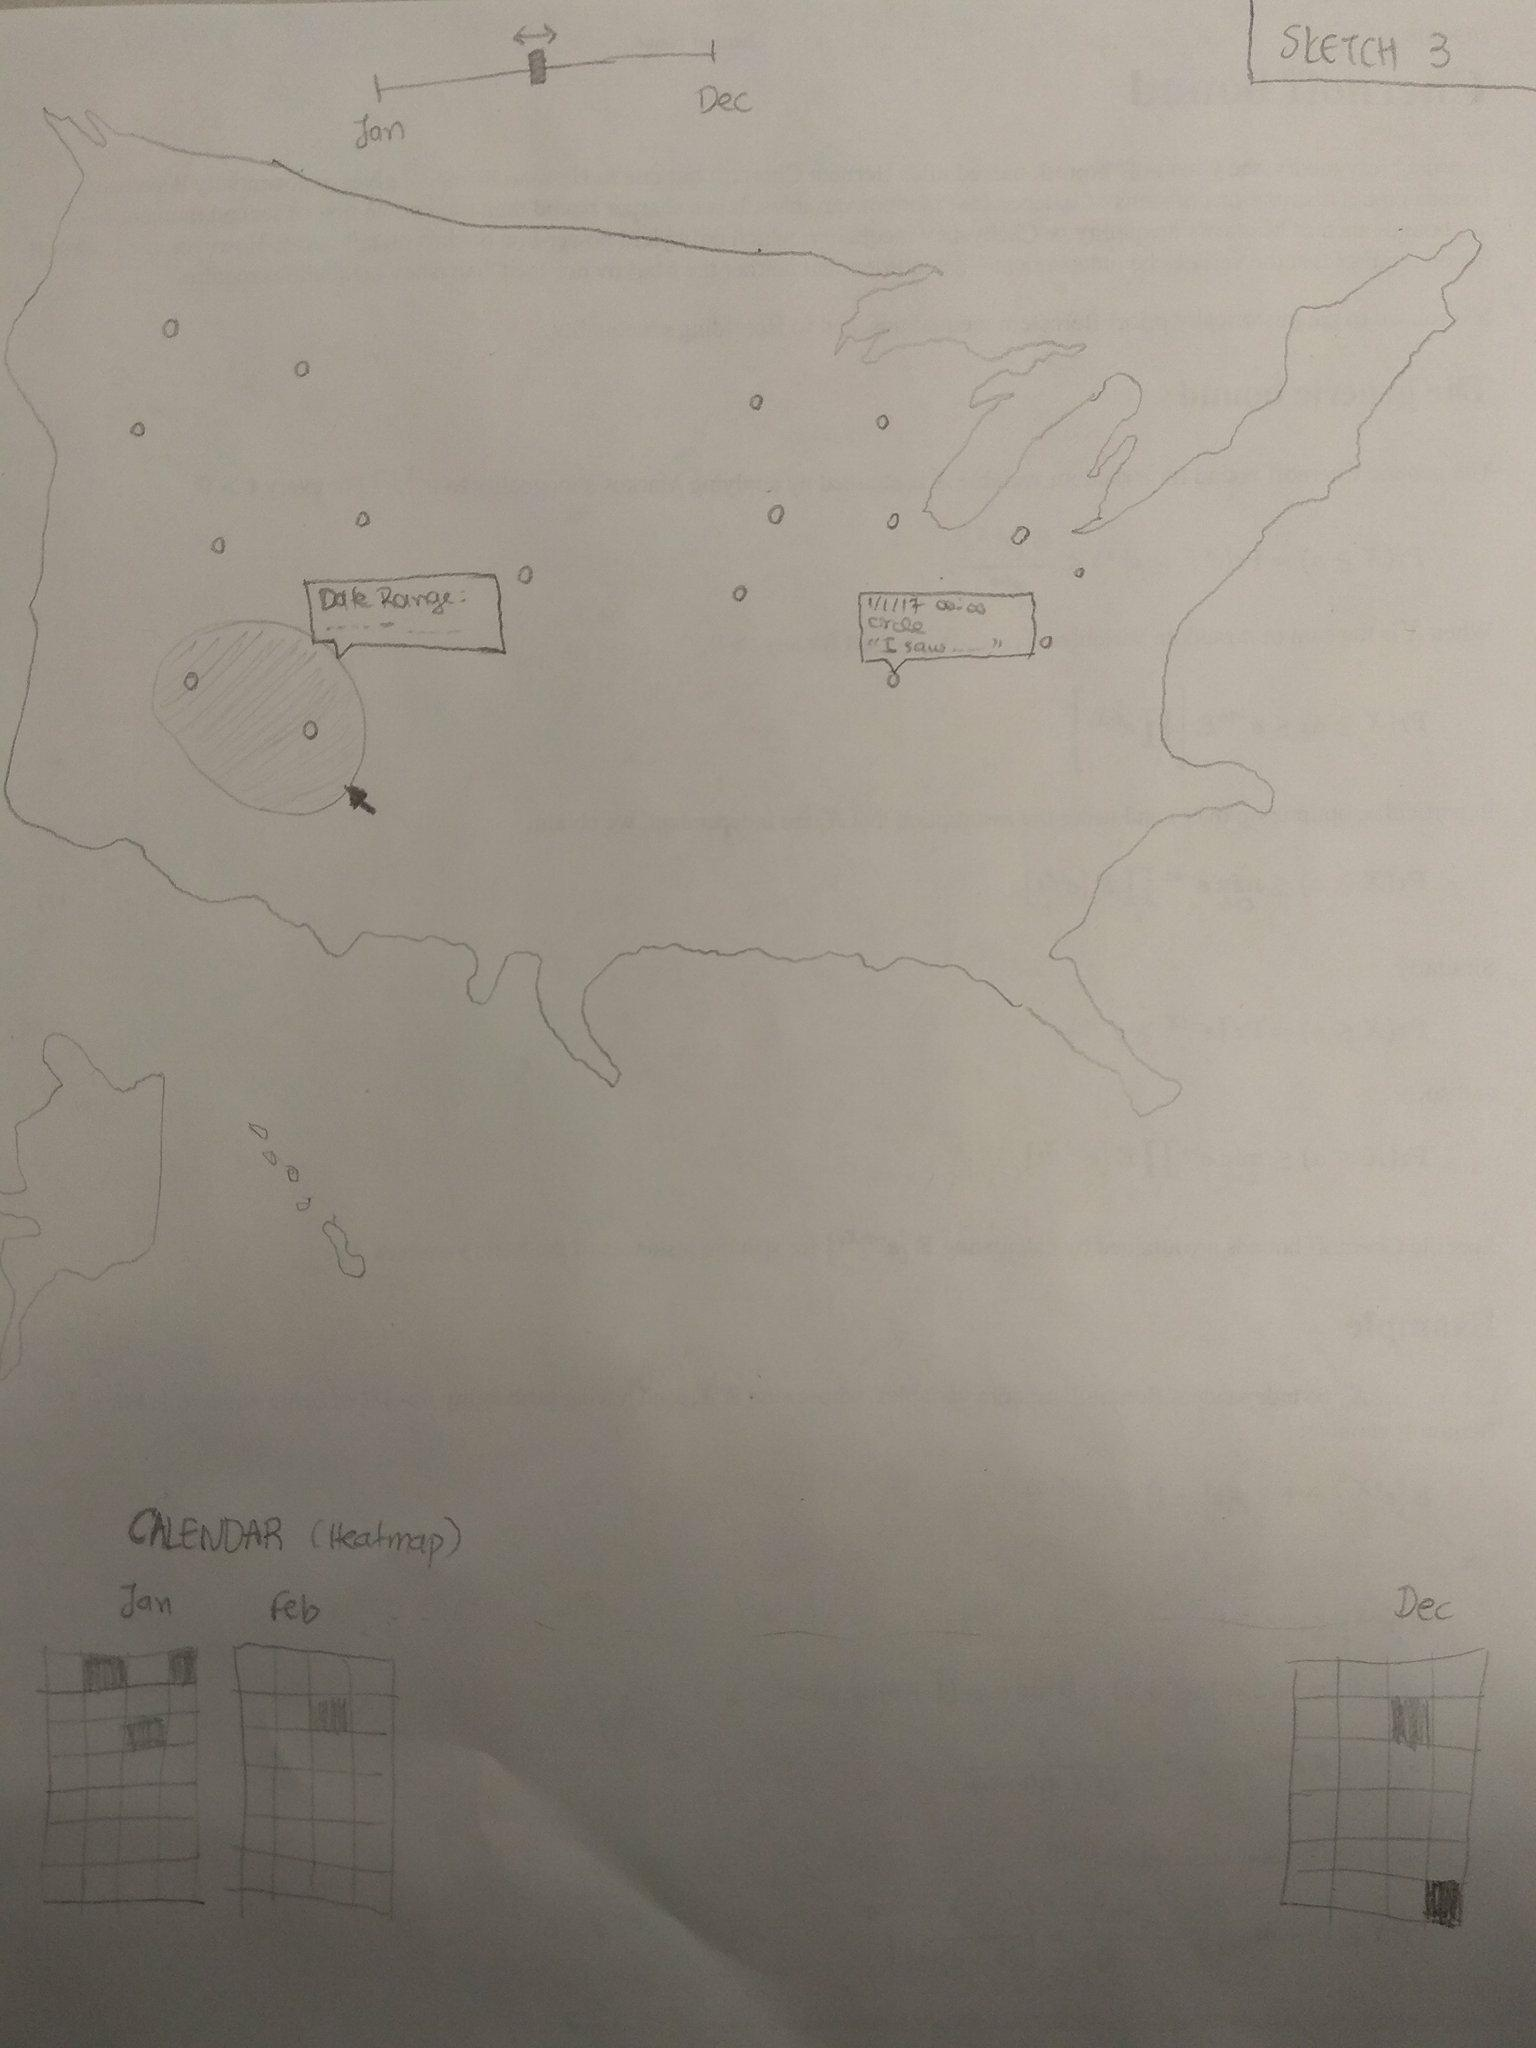
\includegraphics[width=0.7\linewidth]{lydia3}
}
\end{figure}

This visualization supports all 6 most important tasks, as well as the tasks ``When did the sightings of a particular area occur?" (determine range) and ``What date has the most sightings?". This task is now supported by a calendar chart instead of a line chart. Although we are better at perceiving position than color, the calendar map is more enjoyable which makes up for the fact that this visualization is not as interactive as the previous ones.

\newpage

\subsubsection*{4.2.4 Peter's}

\begin{figure}[h]
\centering
{
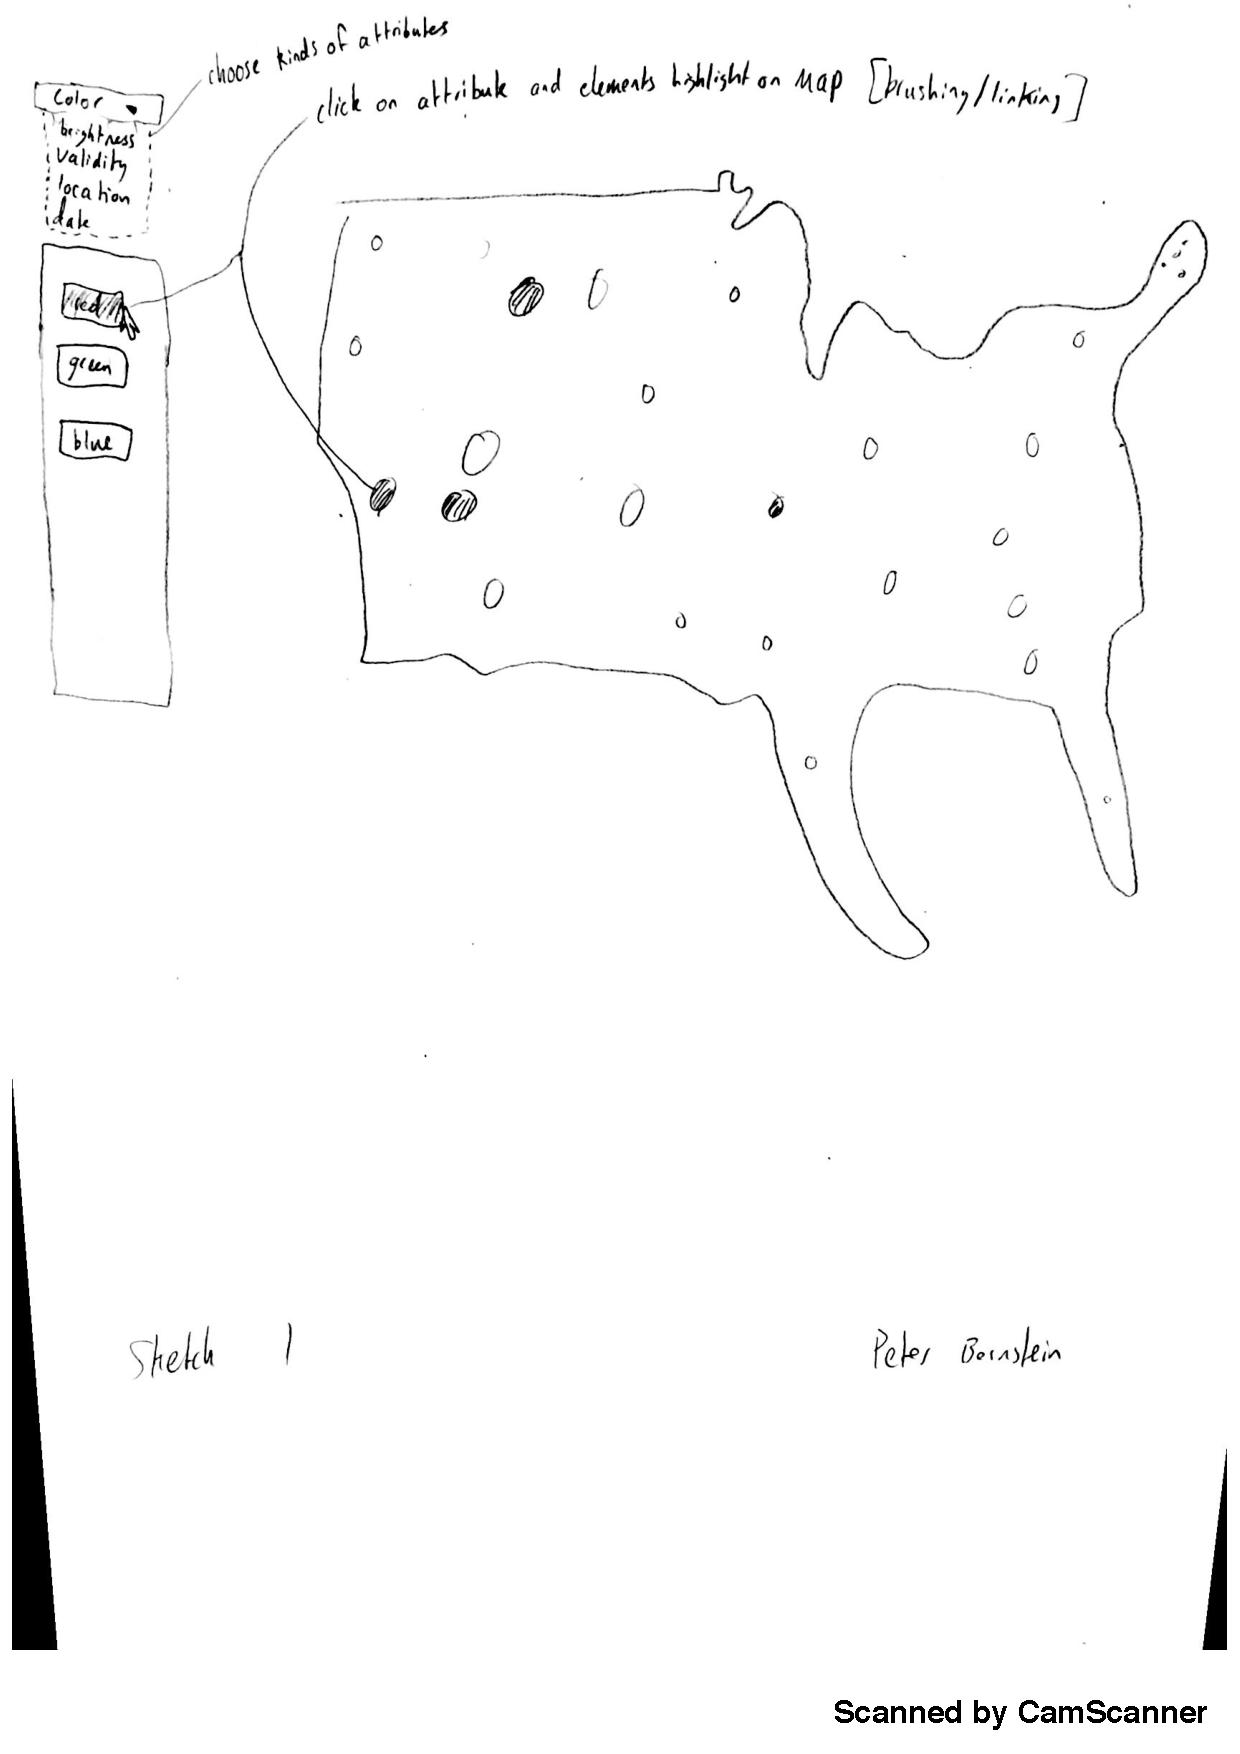
\includegraphics[width=0.7\linewidth]{peter1}
}
\end{figure}

This sketch is motivated by being able to support a variety of different tasks with a dropdown menu on the left. It encodes sightings as dots on a map that can pop out when an attribute that pertains to it is highlighted. \\\\

\newpage

\begin{figure}[h]
\centering
{
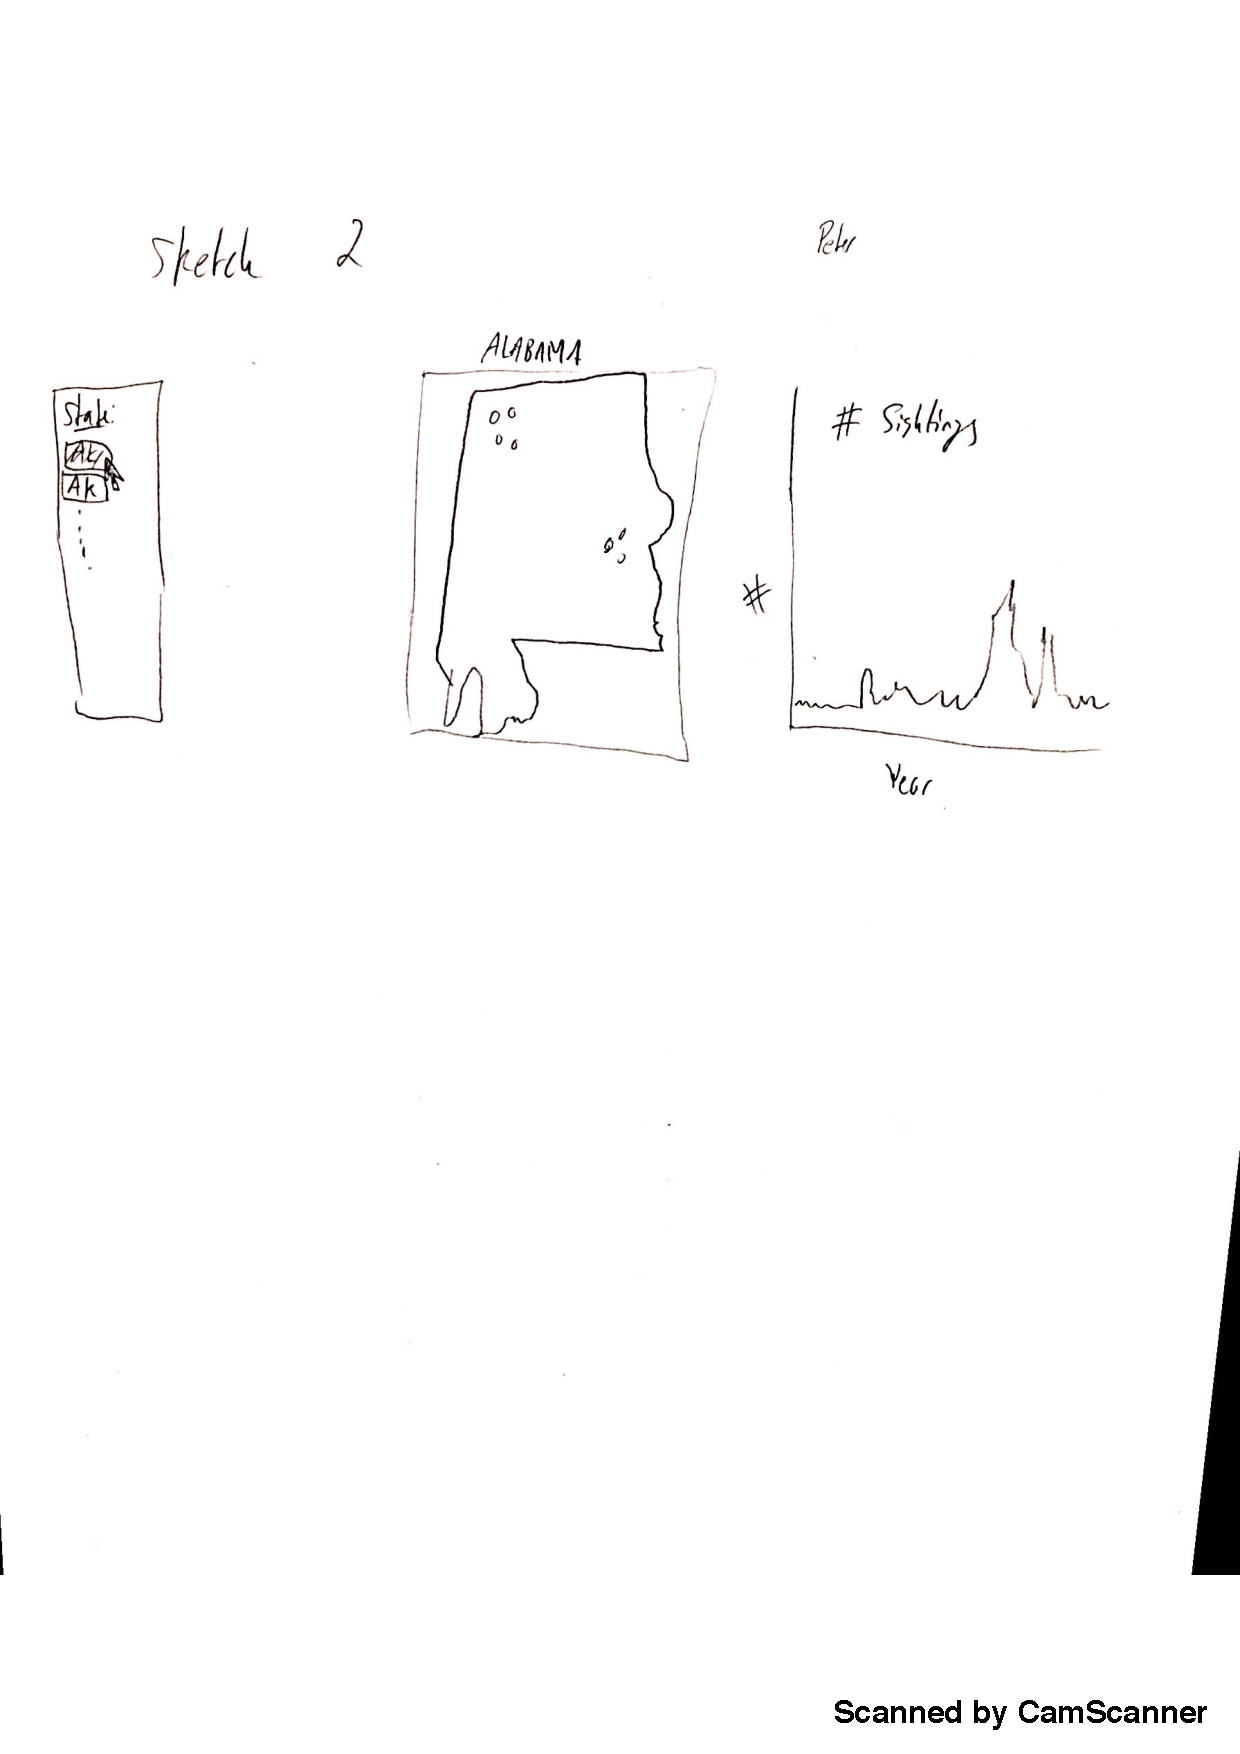
\includegraphics[width=0.7\linewidth]{peter2}
}
\end{figure}
This is motivated by the task of making it easier to retrieve information about sightings. A countrywide map could be overwhelming so breaking it down by states and showing a distribution also tackles the ``characterize distribution" task well.\\\\

\newpage

\begin{figure}[h]
\centering
{
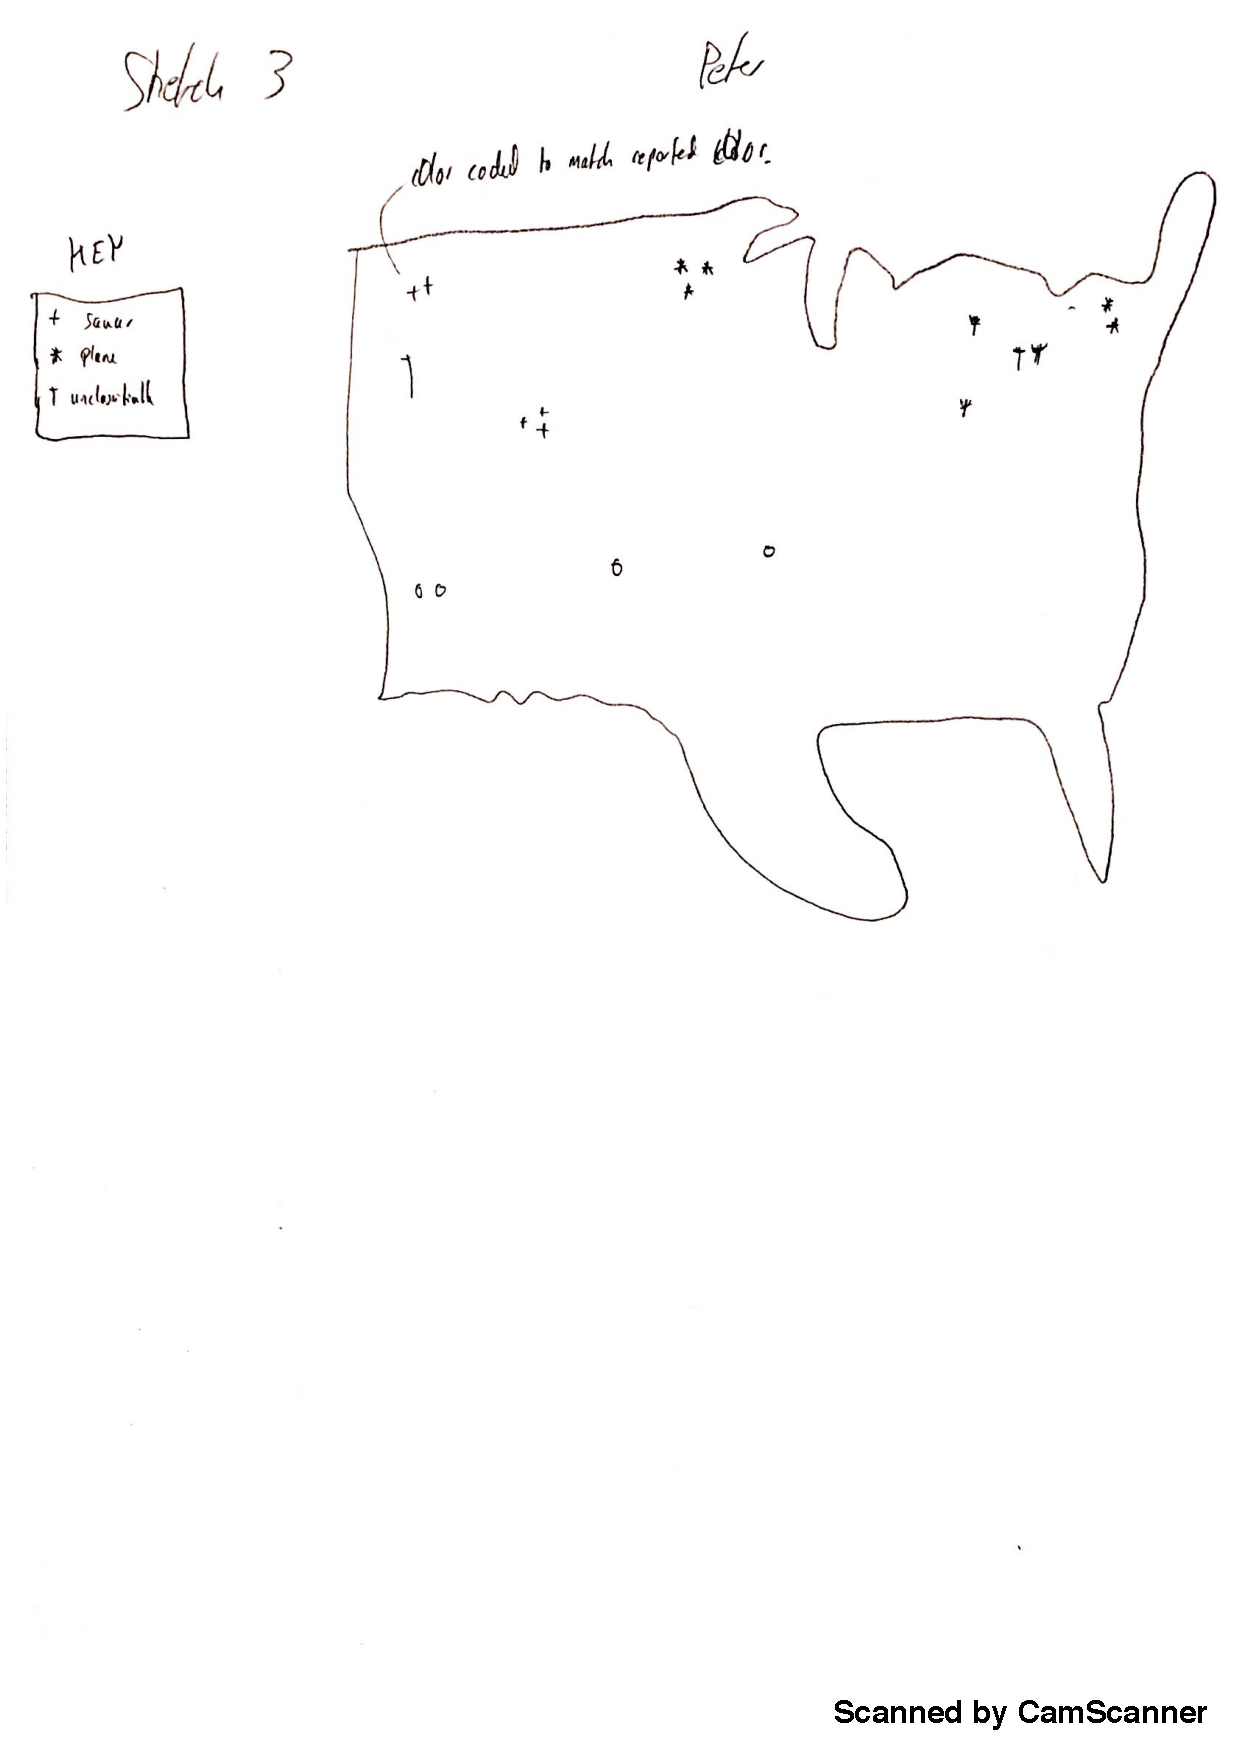
\includegraphics[width=0.7\linewidth]{peter3}
}
\end{figure}
This sketch is designed to help more with the clustering and retrieve value tasks because it would have a visual encoding of the different kinds of sightings immediately visible on the national map. This idea would require a zoom feature to be useful and tooltips as well, but the general idea could be incorporated with others.\\\\

\newpage

\subsection*{5 Group Feedback}

1. Entire U.S. map and then zoom / drill in functionality with left hand panel (Emily's visualization) \\

2. Calendar (Lydia's visualization) \\

3. Sliding data (Abby's visualization)


\end{document}
